\chapter{METODOLOGI}
\label{sec:chap3_metodologi}

\section*{ }
Pada penelitian ini nantinya akan terdiri dari lima langkah utama yaitu :
\begin{figure}[H]
	\centering
	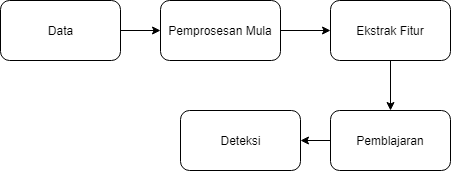
\includegraphics[width=\linewidth]{bab3/BlokDiagram}
	\caption{Blok Diagram Penelitian}
	\label{fig:blokdiagram}
\end{figure}


\section{Data}
Data adalah citra yang diperoleh dari kamera dengan ukuran $300\times 300$ dari beberapa sudut pandang yang berlainan.
\section{Pemprosesan Mula}
Citra yang telah diperoleh telah terpapar oleh gaussia noise sehingga perlu diperbaiki.
\section{Ekstraksi Fitur}
\lipsum[2]
\subsection{Fitur Warna}
\lipsum[1]
\subsection{Fitur Permukaan}
\section{Pembelajaran}
\lipsum[4]
\section{Deteksi}
\lipsum[2]






